\documentclass{beamer}
\usepackage[T1]{fontenc}

%\documentclass[aspectratio=169]{beamer}
%\usetheme{Madrid} % My favorite!
%\usetheme{Boadilla} % Pretty neat, soft color.
%\usetheme{default}
%\usetheme{Warsaw}
%\usetheme{Bergen} % This template has nagivation on the left
\usetheme{Frankfurt} % Similar to the default 
%with an extra region at the top.
\usecolortheme{seahorse} % Simple and clean template
%\usetheme{Darmstadt} % not so good
% Uncomment the following line if you want %
% page numbers and using Warsaw theme%
% \setbeamertemplate{footline}[page number]
%\setbeamercovered{transparent}
\setbeamercovered{invisible}
\setbeamersize{text margin right=3.5mm, text margin left=7.5mm}  % text margin
% To remove the navigation symbols from 
% the bottom of slides%
%
\usepackage{graphicx}
\usepackage[backend=biber]{biblatex}

\addbibresource{PAP14.bib}
\usepackage{tikz}
\usepackage{calc}
\def\checkmark{\tikz\fill[scale=0.4](0,.35) -- (.25,0) -- (1,.7) -- (.25,.15) -- cycle;} 
\def\scalecheck{\resizebox{\widthof{\checkmark}*\ratio{\widthof{x}}{\widthof{\normalsize x}}}{!}{\checkmark}}
%that's defined it - now for a test

\DeclareGraphicsExtensions{.pdf,.png,.jpg}
%\usepackage{bm}         % For typesetting bold math (not \mathbold)
%\logo{\includegraphics[height=0.6cm]{yourlogo.eps}}
%
\title[Trust in Collaborative Marine Networks]{An Investigation into Trust and Reputation Frameworks for Collaborative Teams of Autonomous Underwater Vehicles}

\author{Andrew Bolster}
\institute[UoL]
{
University of Liverpool \\
\medskip
{\emph{andrew.bolster@liv.ac.uk}}\\
\vspace{0.3in}

\includegraphics[width=0.5\textwidth]{img/livuni}%
}
\date{June 4, 2014}
% \today will show current date. 
% Alternatively, you can specify a date.
%
\begin{document}
%

%\AtBeginSection[
%{
%\begin{frame}<beamer>{Table of Contents}
%  \tableofcontents[currentsection,currentsubsection, 
%  hideothersubsections, 
%  sectionstyle=show/shaded,
%  ]
%\end{frame}
%}]
\begin{frame}
  \titlepage
\end{frame}

\frame{\tableofcontents}

\section{Context}
\frame{
\frametitle{Research Context}
\begin{itemize}
  \item Project launched at QUB ECIT in 2011 under the DSTL/DGA Anglo French Defence Research Group PhD Programme  \item What lessons from the Mobile Ad Hoc Network (MANET) space can be transferred to the marine environment?
  \item Teams of 3 - 16 Autonomous Underwater Vehicles (AUVs) Mine countermeasures, Hydrography, and Patrol Capabilities (MHPC)
  \item Defence focus, assumption of highly capable enemy attempting to compromise communications / operations
  \item Primary Simulation/Analysis work done in 12/13
  \item Moved to UoL Oct 13 after 2 mth placement @ DSTL PDW Naval Systems / Information Systems departments.
  \item CDE Project on Precision Timing for Positioning with NPL/Plextek
\end{itemize}
}

\section{Trust in Networks}
\subsection{What do we mean by trust?}
\frame{
\frametitle{Trust in Ad-Hoc Systems and the context of this document}
\begin{itemize}
  \item Particularly interested in the application of Trust in Decentralised (P2P) Autonomous Systems of Systems, Autonomous Underwater Vehicles (AUVs) for example
  \item <2->Trust:\emph{The expectation of an actor performing a certain task or range of tasks within a certain confidence or probability}
  \item<3->Full System Views of Trust
    \begin{itemize}
      \item<3->{Design Trust - that a system of systems will perform as spec'd / designed in operation}
      \item<4>{Operational Trust - the systems within a larger system will perform as designed in field \checkmark}
    \end{itemize}
\end{itemize}
}
\subsection{What are TMFs?}
\frame{
\frametitle{Trust Management Frameworks}
\begin{itemize}
  \item Provide information regarding the estimated future states and operations of nodes within networks
  \item <2->``[\ldots]collecting the information necessary to establish a trust relationship and dynamically monitoring and adjusting the existing trust relationship'' - \cite{Li2007}
  \item <3->Enables nodes to form collaborative \emph{opinions} on their cohort nodes based on
    \begin{itemize}
      \item Direct Observation of Communications Behaviour (eg Successfully Forwarded Packets)
      \item Common-Neighbour Recommendation
      \item Indirect Reputation
    \end{itemize}
\end{itemize}
}
\frame{
\frametitle{Transitivity in Trust Networks}
\begin{center}
  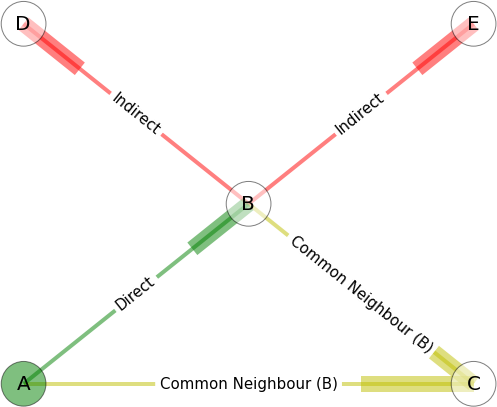
\includegraphics[height=0.6\paperheight]{img/node_relationships}
\end{center}
}

\subsection{Reasons for using Communication TMFs}
\frame{
\frametitle{TMFs in Ad Hoc Autonomous Systems}
\begin{itemize}
  \item Multiple transitive relationships can be maintained over time, providing trust resilience with dynamic network topology
  \item<2->Enable trust establishment from partial-strangers via indirect trust and direct observation
  \item<3->Enables nodes to inform internal processes for global efficiency given observed network behaviour / 'wellness', similar to those found in human social networks eg
    \begin{itemize}
      \item Update routing table based on 'safest' node chains (Phone Tree)
      \item Maneuver away from misbehaving nodes (Shunning)
      \item Inform as to 'trustworthiness' of forwarded information (Healthy sense of Skepticism)
      \item Historic Distrust/Trust decaying over time (Forgiveness/Relationship Decay)
    \end{itemize}
\end{itemize}
}
\frame{
\frametitle{Reason for using TMFs in MANETs}
\begin{itemize}
  \item Provide Risk Mitigation against many classical MANET attacks
    \begin{itemize}
      \item Black/Grayhole
      \item Routing Loop
      \item Selective misbehaviour / selfishness
    \end{itemize}
  \item Generally; to constrain potential malicious behaviour that can operate without detection
\end{itemize}
}

\subsection{Pre-existing Research}
\frame{
\frametitle{Trust in Autonomous Systems}
\begin{itemize}
  \item Public Key Infrastructure - Requires Centralised Control and pre-shared keys
  \item Resurrecting Duckling - Uses in-action keying with a trusted source
  \item Evidence Based Trust - Uses shared keys 
  \item Reputation Based Trust - Uses Packet forwarding success rate for prediction of future actions
    \begin{itemize}  
      \item CONFIDANT - Trust-based router implementation using packet forwarding rate
      \item OTMF - Trust including transitive information from other nodes
      \item <2-> MPTM - Relationships and Multiple Metrics combined with Gray Interval assessment
    \end{itemize}
  \item \ldots and there are plenty more along the same lines
  \item Predominantly use single metrics or only communications metrics
\end{itemize}
}


\section{Fusions of Trust Metrics}
\subsection{Vector Trust}
\frame{
\frametitle{Vectorised Trust}
\begin{itemize}
  \item Application of several individual metrics for the construction of a single trust measurement
  \item For example:
    \begin{itemize}
      \item $X=\{packet\ loss, signal\ strength, data rate, delay, throughput\}$
    \end{itemize}
  \item This multi-parameter trust prevents 'smart' attackers; leveraging a known trust metric to subvert a TMF without detection
  \item Normally expressed as a vector, but can be condensed into an abstracted or weighted form for comparison \cite{Guo}
\end{itemize}
}
\frame{
\frametitle{The Need for Multi-Domain Trust Assessment}
\begin{itemize}
  \item Communications not the only target for an attacker (or failure);
    \begin{itemize}
        \item Following to restricted area
        \item Masquerading
        \item Hardware Degradation
        \item Resource attack via propulsive power
    \end{itemize}
  \item Physical observation presents opportunity to further reduce the available threat surface while also discriminating between 'True' attacks and mechanical failure.
  \item Also could provide additional 'handshake' protocols for 'friendly' fleets/teams through reactionary behaviours
\end{itemize}

}
\frame{
\frametitle{Multi-Vector Trust and the Threat Surface}
Potential attacks exist across a multi-domain threat surface
\begin{center}
  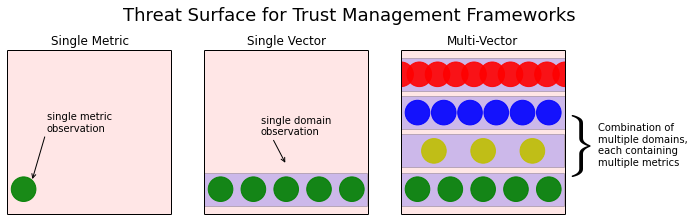
\includegraphics[width=0.9\paperwidth]{img/threat_surface_sum}
\end{center}
}


\frame{
\frametitle{Malicious Behaviour Discrimination}
\begin{center}
  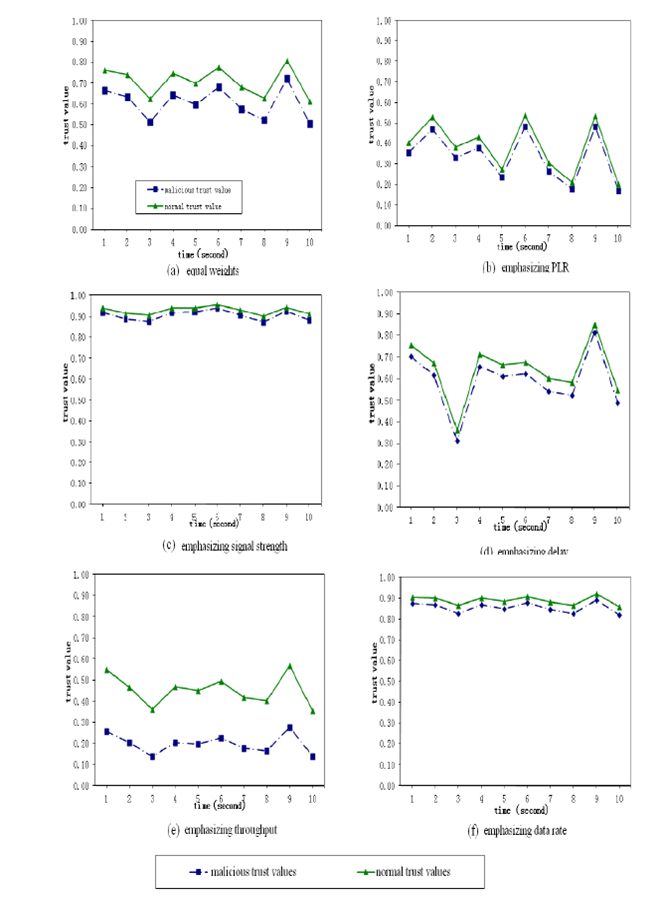
\includegraphics[height=0.8\paperheight]{img/bellas_vector_detector}
\end{center}
}



\subsection{Multi-Vector Trust}
\frame{
\frametitle{Agent Based Behaviour Simulator}
\begin{center}
  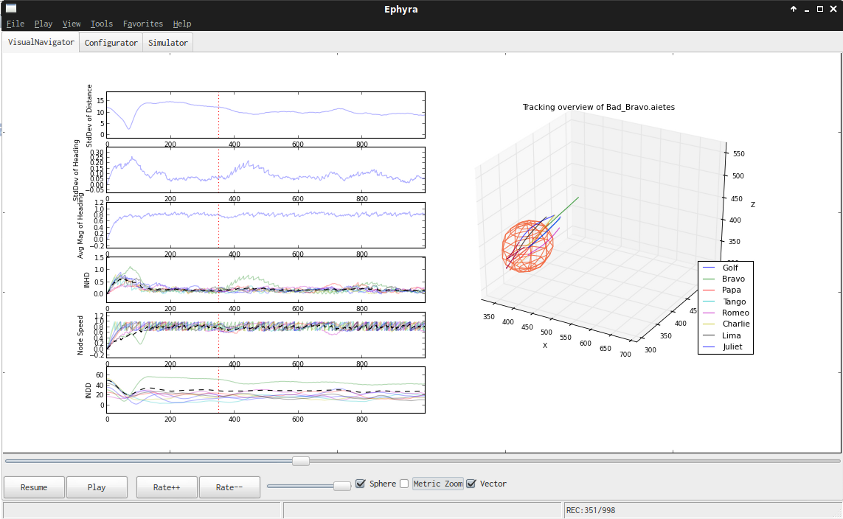
\includegraphics[width=0.9\paperwidth]{img/ephyra_vis}
\end{center}
}

\frame{
\frametitle{Trust in Mobile Autonomous Underwater Vehicles}
\begin{itemize}
  \item Flocking with Intent: MCM, Port Protection, Survey, Protection Detail, etc.
  \item<2-> Metric Selection in collaboration CMRE/DSTL
    \begin{itemize}
      \item Inter Node Heading Deviation
      \item Inter Node Distance Deviation
      \item Node Speed
    \end{itemize}
  \item <3-> Behaviour selection for testing
    \begin{itemize}
      \item Shadow
      \item Spy
      \item Sloth
      \item Stalker
      \item Scoundrel
      \item <4-> Slow Coach (non-malicious)
      \item <4-> Spin Doctor (non-malicious)
    \end{itemize}

\end{itemize}
}
\frame{
\frametitle{Raw Behavioural Metric Assessment in AUVs}
\begin{center}
  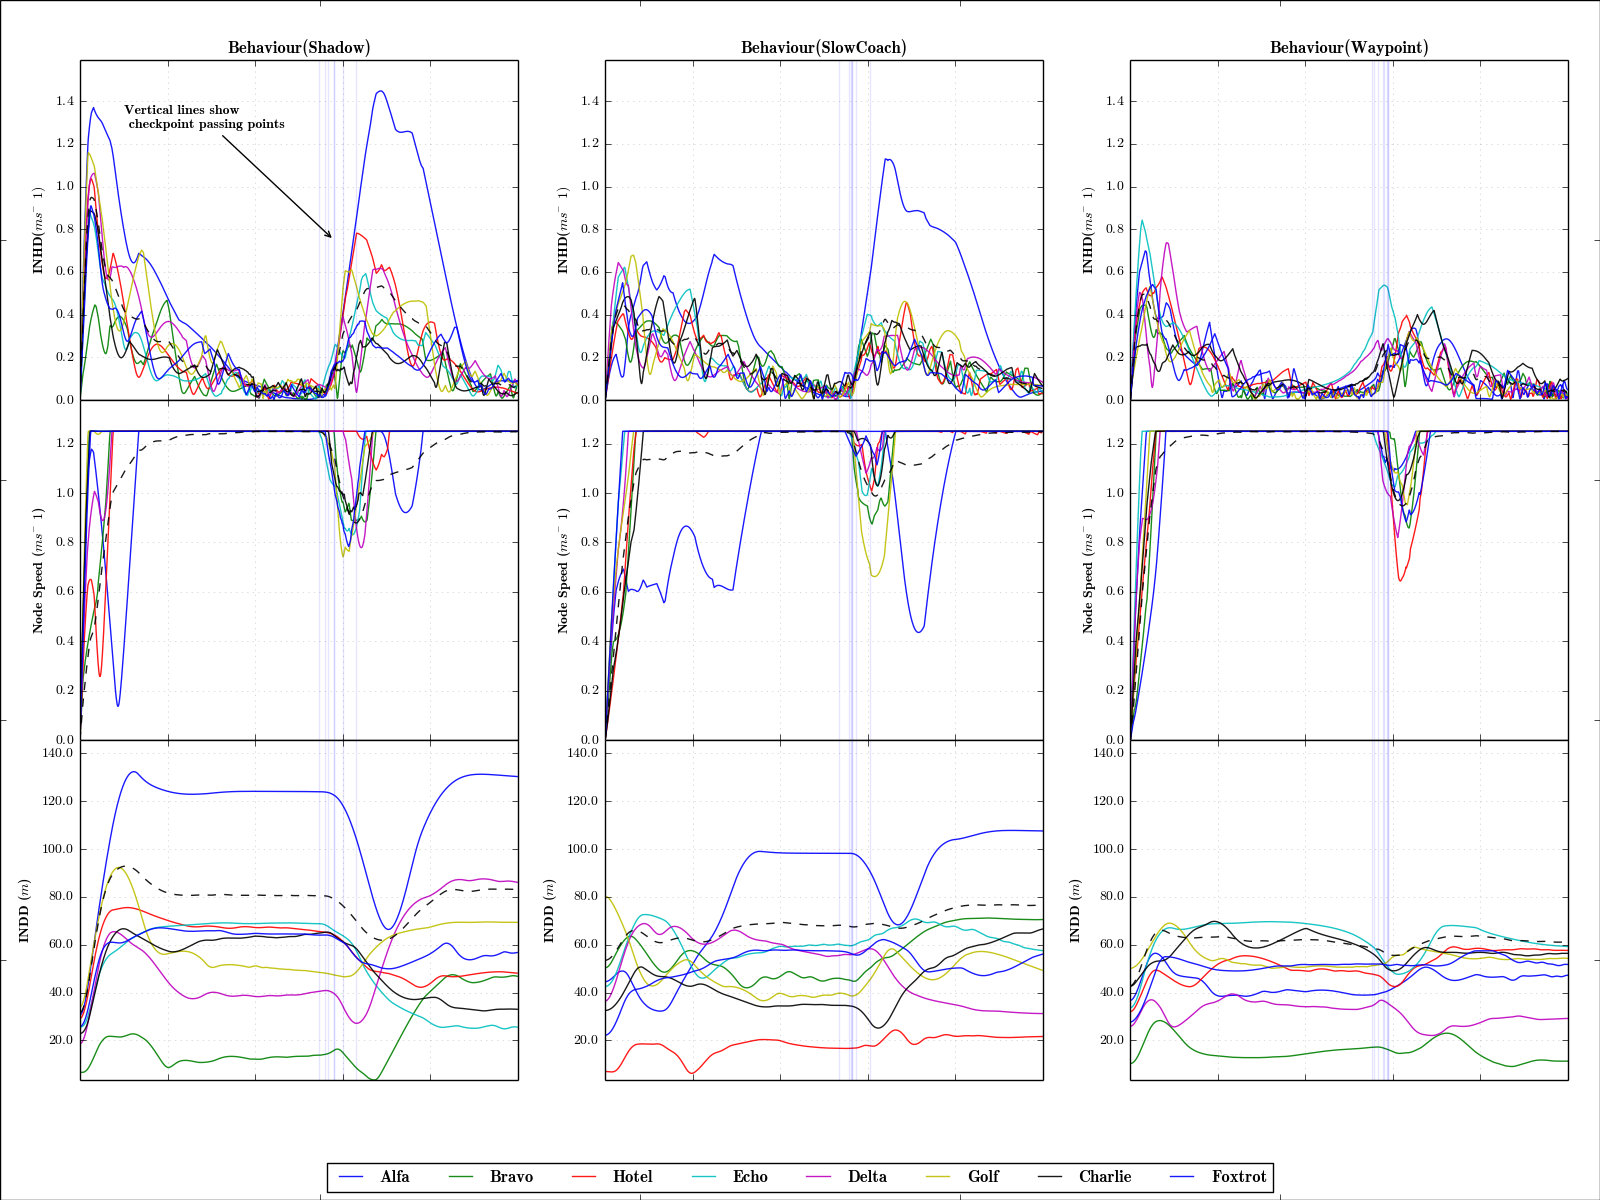
\includegraphics[height=0.8\paperheight]{img/BehaviourMetricComparison}
\end{center}
}
\frame{
\frametitle{Behavioural Trust Assessment in AUVs}
\begin{center}
  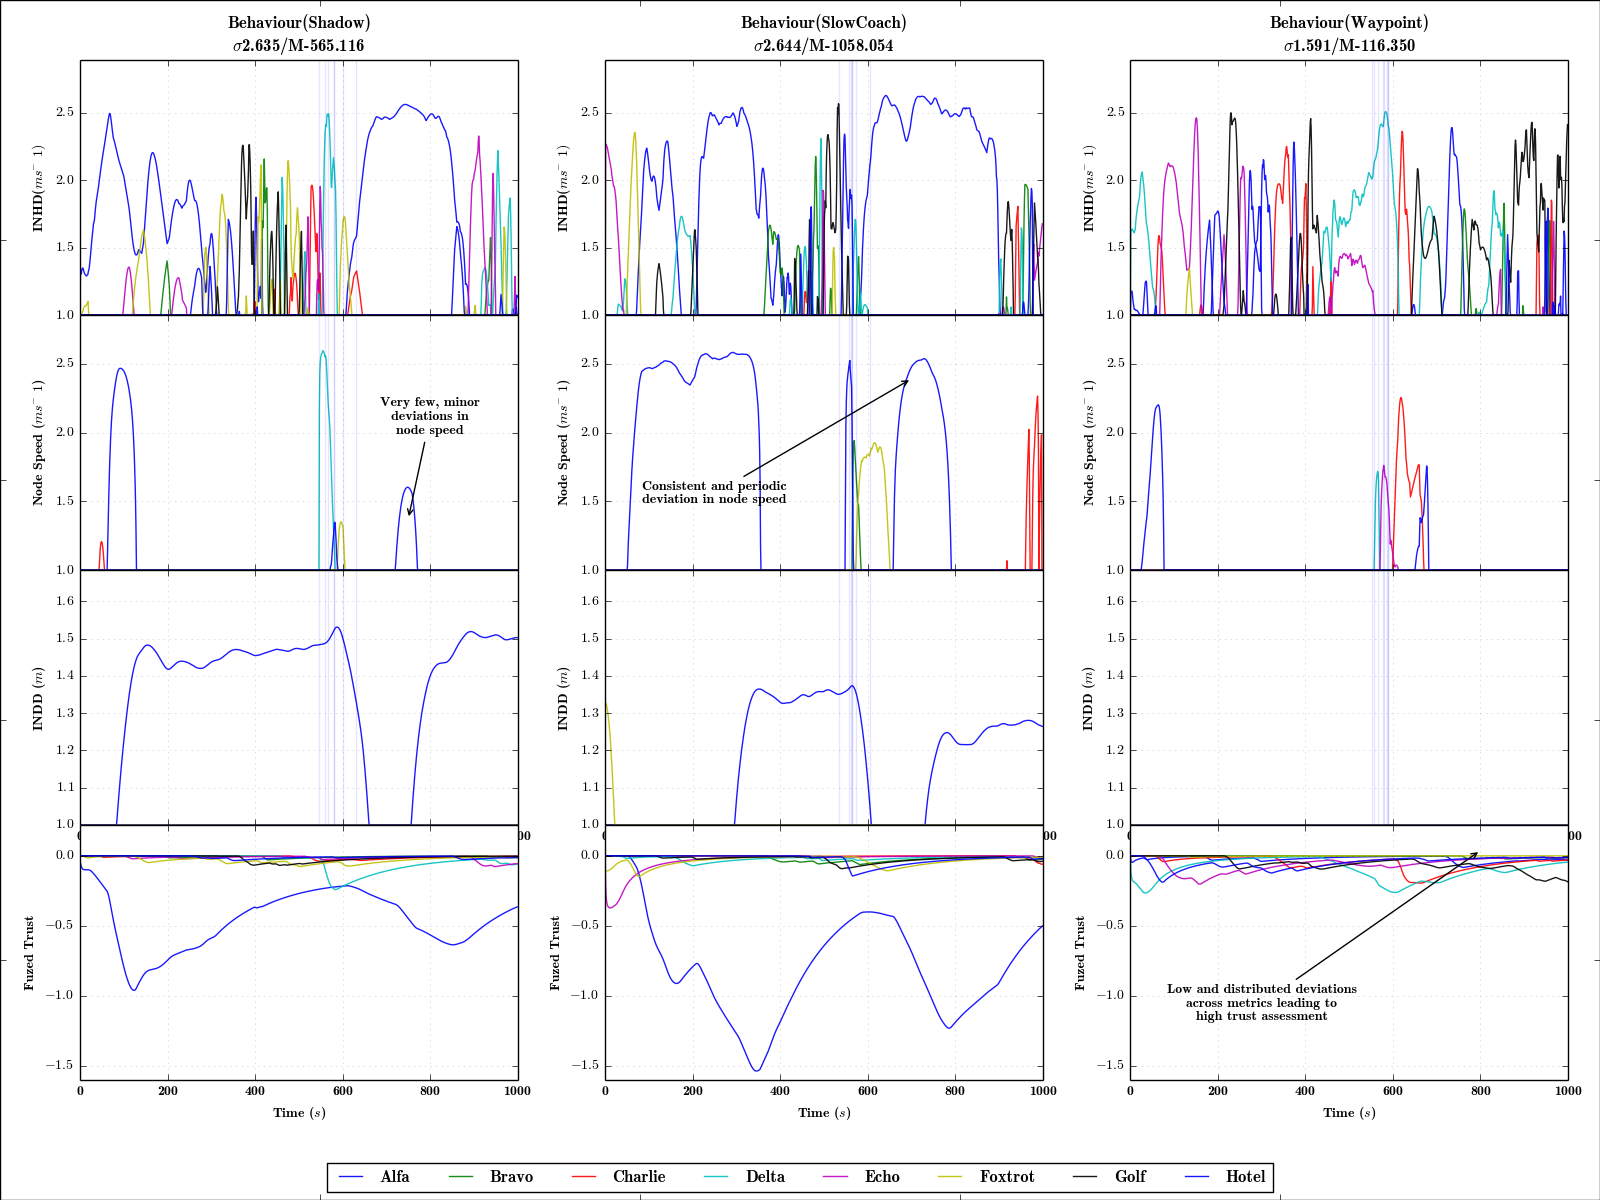
\includegraphics[height=0.8\paperheight]{img/BehaviourFusion}
\end{center}
}
\frame{
\frametitle{Behavioural Trust Assessment in AUVs}
\begin{itemize}
  \item Detection and identification based on basic weight-assessment classifier against windowed history of observations, with confidence based on a Grey Theoretic weight
  \item Currently >96\% statistical accuracy of detection and confidence, but this needs much more rigorous analysis

\end{itemize}
}
\subsection{Challenges for Implementing Multi-vector Trust}
\frame{
\frametitle{Challenges in Multi-vector Trust}
\begin{itemize}
  \item How to define optimality in trust assessment when dealing with multiple vectors and transitive trust?
  \item Is there a quantifiable benefit to cross-domain comparison beyond single vector Trust?
  \item Is there an optimal generic cross-domain comparator?
\end{itemize}
}

\section{Development Plan}
\subsection{Publications}

\frame{
\frametitle{Current Publications}
\begin{itemize}
\item A Multi-Vector Trust Framework for Autonomous Systems \cite{Bolster2014}
  \begin{itemize}
  \item Symposium paper to the Association for the Advancement of Artificial Intelligence on the current state of work, presenting our progress towards multi-vector trust
  \end{itemize}


\item Analysis of Trust Interfaces in Autonomous and Semi-Autonomous Collaborative MHPC Operations \cite{Bolster2014a}
  \begin{itemize}
  \item Part of a Five-Eyes defence strategy programme (TTCP) for assuring C3I capabilities as part of FF2020
  \end{itemize}


\end{itemize}
}

\frame{
\frametitle{Development Plan}
\begin{enumerate}
  \item Behaviour Detection (Q3 14) - Formal Analysis of Behavioural Trust Systems
  \begin{itemize}
    \tiny
    \item ASON 2014 : Seventh Int. WS on Autonomous Self-Organizing Networks (Aug 14)
    \item AHUC 2014 : The Fourth Int. WS on Ad Hoc and Ubiquitous Computing (Aug 14)
    \item ICCAR 2015 : WASET Int. Conf. on Control, Automation and Robotics (Dec 14)
  \end{itemize}
  \item MANET/Marine comparison (Q4 14) - Formal Comparison between Terrestrial MANET / Marine contexts
  \item Multi-Domain Trust Assessment (Q4 14) - Combination of Communicative and Physical Behaviour Trusts
  \begin{itemize}
    \tiny
    \item IEEE Trans. on Communications / Dependable and Secure Computing / Intelligent Systems
  \end{itemize}
  \item Reactionary/Perturbative Trust (Q1 15) - Exploration of reactionary behaviours for teams to 'shake down' suspects
  \begin{itemize}
    \tiny
    \item SASO15:Self-Adaptive and Self-Organizing Systems, 
    \item SEAMS15: Software Engineering for Adaptive and Self-Managing Systems
  \end{itemize}
\end{enumerate}
}


\subsection{Thesis Plan}
\frame{
\frametitle{Thesis plan}
\begin{itemize}
  \item Abstract, Acknowledgements, Introduction, 
  \item Background Information on Trust and it's applications to MANETs
  \item Background Information on Maritime Uses of Autonomous Systems
  \item Trust in Autonomous Systems of Systems for Maritime Defence Applications
  \item Strategies for Multi-Domain Trust Assessment
  \item Modelling and Analysis of Collaborative Node Kinematic Behaviours in Underwater Acoustic MANETS
  \item Comparative Analysis of Multi-Domain Trust Assessment in Collaborative Mobile Networks
  \item Reactionary Behaviours to increase decentralised trust in isolated environments
  \item Conclusions, Bibliography
\end{itemize}
}

%
\begin{frame}[t,allowframebreaks]
  \frametitle{References}
  \printbibliography[title=References]% [nottype=video]}
\end{frame}

\begin{frame}
  \centerline{The End}
\end{frame}
% End of slides
\end{document} 


